\section[Cooling effectiveness]{Overall Effectiveness: Four Objectives, an Explicit Choice}
\label{sec:effectiveness}

\subsection{Performance, access, energy and cost}
We retain the physical outputs and compare four quantities,
\begin{equation}
 \min_s\big(\overline R_s,\ X_s,\ E_{s,y},\ C_{s,y}\big),\qquad
 X_s=\frac{\sum_{z,k}x_{zk}b_k}{\sum_z A_z}.
\label{eq:effectiveness-vector}
\end{equation}
Remaining SET excess measures thermal performance. $X_s$ is the fraction of dining area reserved for equipment and maintenance clearance, providing a calculable \textit{visitor-access proxy}. Clear walkways and exits remain layout requirements. $E_{s,y}$ measures resource use, and $C_{s,y}$ measures annual expenditure. Thermal relief is counted once; $\eta$ is not a fifth objective.

All ownership, maintenance and running costs use the annual basis in Table~\ref{tab:venue-inputs}. With capital recovery factor $\operatorname{CRF}=r(1+r)^L/[(1+r)^L-1]$,
\begin{equation}
 \begin{aligned}
 C_{s,y}&=\operatorname{CRF}\sum_{z,k}x_{zk}K_k+
             \sum_{z,k}x_{zk}M_k+\pi_eE_{s,y}+\pi_wV_{s,y},\\
 V_{s,y}&=\frac{3600H_y\lambda_w}{\rho_w}
          \sum_{z,k}x_{zk}\dot m_k(w_{e,k}-w_a).
 \end{aligned}
\label{eq:venue-cost}
\end{equation}
Here $K_k$ and $M_k$ are initial and annual maintenance costs, $H_y$ is annual operating hours, and $\rho_w$ converts evaporated mass to water volume. The common USD price basis supports comparison. EIA's Arizona commercial average, USD $0.1245$/kWh in 2025 \cite{eia-commercial}, falls within the electricity sensitivity range.

\subsection{Conditional recommendations from the full candidate set}
For Task 4, we impose the assumed coverage requirement, then remove four-objective dominated options. Phoenix/Singapore have $199/106$ eligible count combinations and $80/32$ \textbf{coverage-constrained Pareto options}. For identical counts, energy, cost and clearance are position-independent here; retaining the eligible layout with least residual therefore preserves the policy optimum. Under an illustrative operator policy,
\begin{equation}
 s^*=\arg\min_s C_{s,y}\quad\text{subject to}\quad
 q_s\ge q_{\min},\quad\overline R_s\le\overline R_{\max},\quad
 X_s\le X_{\max},\quad E_{s,y}\le E_{\max}.
\label{eq:effectiveness-selection}
\end{equation}
The limits in Table~\ref{tab:venue-inputs} express a budgeted service choice without arbitrary equal weighting. Exhaustive enumeration establishes the minimum within the discrete design space.

\begin{table}[!ht]
\centering\small
\caption{Selected plans under the stated four-objective policy. Annual costs include ownership, maintenance, electricity and water.}
\label{tab:venue-decisions}
\begin{tabular}{@{}llrrrrr@{}}
\toprule
Venue & Plan & $q$ (\%) & $\overline R$ ($^\circ$C) & $X$ (\%) & $E_y$ (kWh) & $C_y$ (USD)\\
\midrule
Phoenix & A10C2 & 96.67 & 4.482 & 2.67 & 4500 & 3360\\
Singapore & A10 & 90.00 & 7.453 & 2.08 & 1500 & 1293\\
\bottomrule
\end{tabular}
\end{table}

In Phoenix, place two C units and one A in the busiest zone, five A units in the second, and four A in the third. This A10C2 layout delivers $1248.87$ person$\cdot{}^\circ$C$\cdot$h per session using $30$ kWh and $0.319$ m$^3$ of make-up water. A15 is cheaper but misses the residual requirement; C6 exceeds the energy budget. In Singapore, the A allocation $(4,4,2)$ meets the policy with $971.22$ service units and $10$ kWh. Its ten fans require no evaporative make-up water. The different choices emerge from the constraints and climate response.

\begin{figure}[!ht]
\centering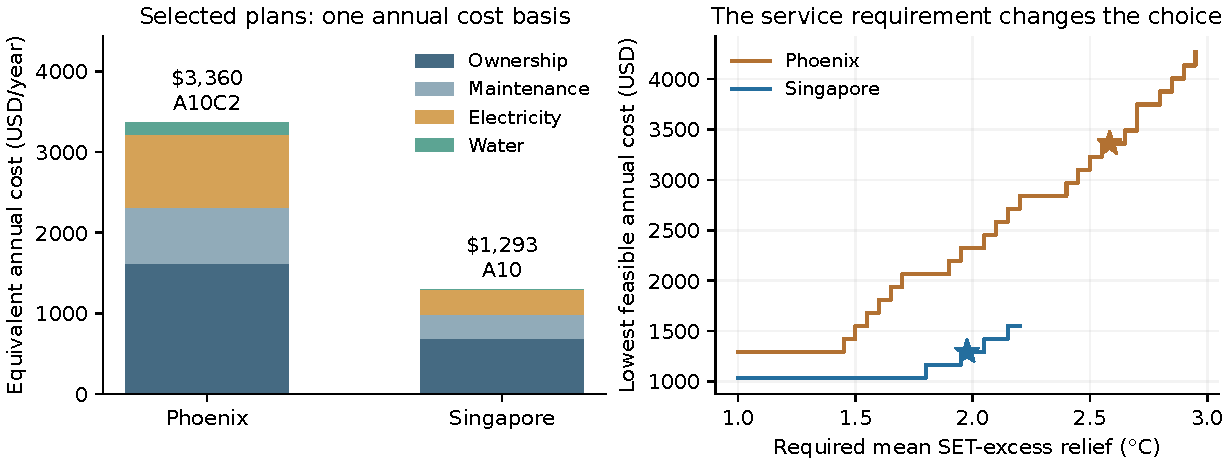
\includegraphics[width=\linewidth]{figures/28_effectiveness.pdf}
\caption{Annual costs of the selected plans and the minimum cost as the required thermal relief increases, holding the other policy limits fixed. Stars mark the stated policy. Stepped curves reflect integer equipment choices.}
\label{fig:venue-effectiveness}
\end{figure}

\subsection{Sensitivity leads to an operating policy}
Across $243$ price combinations, Phoenix retains A10C2 in $228$ ($93.8\%$) and selects A4C3 in $15$; Singapore retains A10 throughout. Physical changes have stronger effects in these tests. A $0.15$ loss in evaporative delivery fraction selects A6C3 in Phoenix; a $20\%$ loss in induced speed selects A7C3 there and A12 in Singapore. Raising RH by ten percentage points leaves both venues without a feasible layout under their unchanged service, access and energy policies. Operators should then revise timing, radiant exposure or the service budget and reoptimize. The memorandum translates these triggers into operating actions.
